% Working chapter, 2026-10-24. Author-confirmed publication-equivalent arXiv v4 compared; see evidence ledger.
% Evidence ledger: planning/verification-gorag.md. Do not designate this chapter final.
\chapter{Adaptive Graph Retrieval for Dynamic Classification with GORAG}
\label{ch:gorag}

This chapter is based on \emph{GORAG: Graph-based Online Retrieval Augmented Generation for Dynamic Few-shot Social Media Text Classification}, published in the Proceedings of the ACM Web Conference 2026~\cite{gorag-paper}. It studies the selection and maintenance of label evidence when a classification task acquires new classes over several rounds. The central question is how a language model can receive a query-specific candidate set while the evidence connecting text to labels changes over time.

\section{Dynamic Few-shot Classification}
\label{sec:gorag:task}

A classification label defines a decision that an application asks a model to make. When the application adds a more specific category, the decision changes even if the underlying language model stays fixed. For example, a social media classification task can initially distinguish threatening language and later introduce identity insults. A model must then distinguish the new label from earlier labels using the available annotated examples. The difficulty concerns both learning the meaning of a new category and keeping the current alternatives visible during prediction.

Few-shot classification supplies a small number of labeled examples for each class. Dynamic few-shot classification adds classes in successive rounds~\cite{gorag-xia-etal-2021-incremental}. The size of the label universe therefore grows independently of the number of examples available for each label. A retrieval system must update its evidence source as classes arrive, and each prediction must refer to the label set available at that round. This setting differs from repeatedly evaluating a fixed classifier on an unchanged collection of labels.

The task also exposes a limitation of simply placing more material in a language model's context. Additional examples provide information about labels, but a larger context can contain many examples that have little bearing on the current text. The candidate list itself grows as classes accumulate. Selecting text passages without narrowing the associated label alternatives leaves the model with a long classification instruction. GORAG therefore treats the selection of candidate labels as an explicit retrieval problem.

The index used in this chapter is a weighted graph of keywords and labels. A keyword can occur in examples from several classes. Its incident edges record these associations, and their costs distinguish how the term is represented in the indexed corpus. The graph allows several query keywords to be considered jointly. A label can participate in the connection between query keywords even when examining one keyword in isolation would give an ambiguous set of alternatives. The retrieved label set depends on the query terminals and the current graph.

GORAG also updates its index after classifying an unlabeled query. Keywords that were absent from the index can then become available to later queries. The predicted label associates the newly observed keywords with a class for subsequent retrieval. Support examples initialize the graph using their supplied labels.

The research question has three connected parts. First, how should a small support set become a graph whose edges distinguish keyword--label associations? Second, how should the graph select a different candidate set for each text as the label universe expands? Third, how can observations from previously classified texts enlarge the index? The following sections develop these operations and then examine their reported classification and resource results.

\begin{figure}[tbp]
\centering
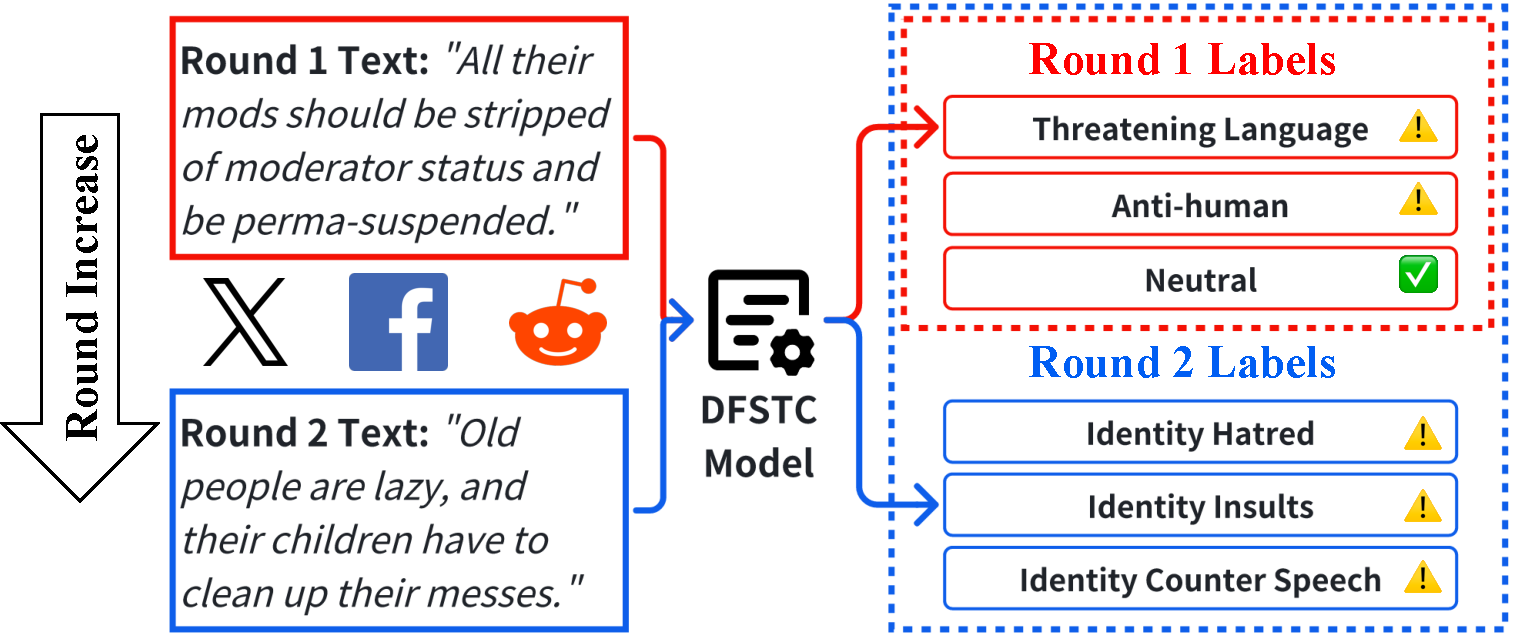
\includegraphics[width=0.9\linewidth]{figures/gorag/DFSTC_task.pdf}
\caption{Two rounds of the dynamic classification task. New abuse categories extend the available labels. Reproduced from Figure 1 of GORAG~\cite{gorag-paper}.}
\label{fig:gorag:task}
\end{figure}

\subsection{Rounds and information availability}
\label{sec:gorag:rounds}

Let $\mathcal{Y}_{\mathrm{new}}^r$ denote the labels introduced at round $r$. The current label universe is
\begin{equation}
\mathcal{Y}^r=\bigcup_{i=1}^{r}\mathcal{Y}_{\mathrm{new}}^i.
\label{eq:gorag:labels}
\end{equation}
The few-shot support data provide $k$ annotated texts per class, with $k$ equal to 1, 5, or 10 in the main experiments. A query text $t$ must be assigned a label from $\mathcal{Y}^r$. The superscript $r$ identifies the current classification round.

For clarity, the support collection visible at a round and the current query stream are separate objects. Support texts carry supplied labels. Query texts become visible as the system processes them, and their predictions can be used for subsequent index updates. Corpus statistics used in keyword scoring refer to training and query texts seen so far. The online association nevertheless inherits prediction errors when the classifier chooses an incorrect label.

Semantic label names supply another source of information. Where names are available, GORAG uses a language model to generate representative descriptions or keywords for labels. These descriptions enter the classification context, and label-derived keywords can support graph initialization. The zero-shot experiment later in this chapter uses this source without any labeled examples. It should therefore be read as a distinct initialization protocol rather than as a smaller support sample from the few-shot experiment.

\section{Weighted Graph Indexing}
\label{sec:gorag:indexing}

GORAG maintains an undirected weighted graph $\mathcal{G}^r=(\mathcal{V}^r,\mathcal{E}^r,\mathcal{W}^r)$. Its node set contains keyword nodes and label nodes. A keyword node represents an extracted word or short phrase. A label node represents a target class. The representation places label alternatives inside the same structure that stores their lexical associations. Support documents contribute keyword--label associations to this representation.

A keyword--label edge is introduced when a keyword occurs in a text associated with that label. Repeated occurrences across texts contribute to the edge weight. A keyword shared by several classes can therefore have several label neighbors, with a different cost for each association. Query retrieval will use these costs when choosing connections between mapped keywords. 

This representation separates the unit used to store evidence from the unit used to make the final prediction. The graph stores keyword--label associations. The language model receives the original query text as well as the retrieved alternatives and their descriptive information. The model can use syntactic and contextual information from the whole query even when retrieval has operated on a smaller collection of keywords. The keyword-only ablation examines the consequence of removing this full-text component.

\begin{figure}[tbp]
\centering
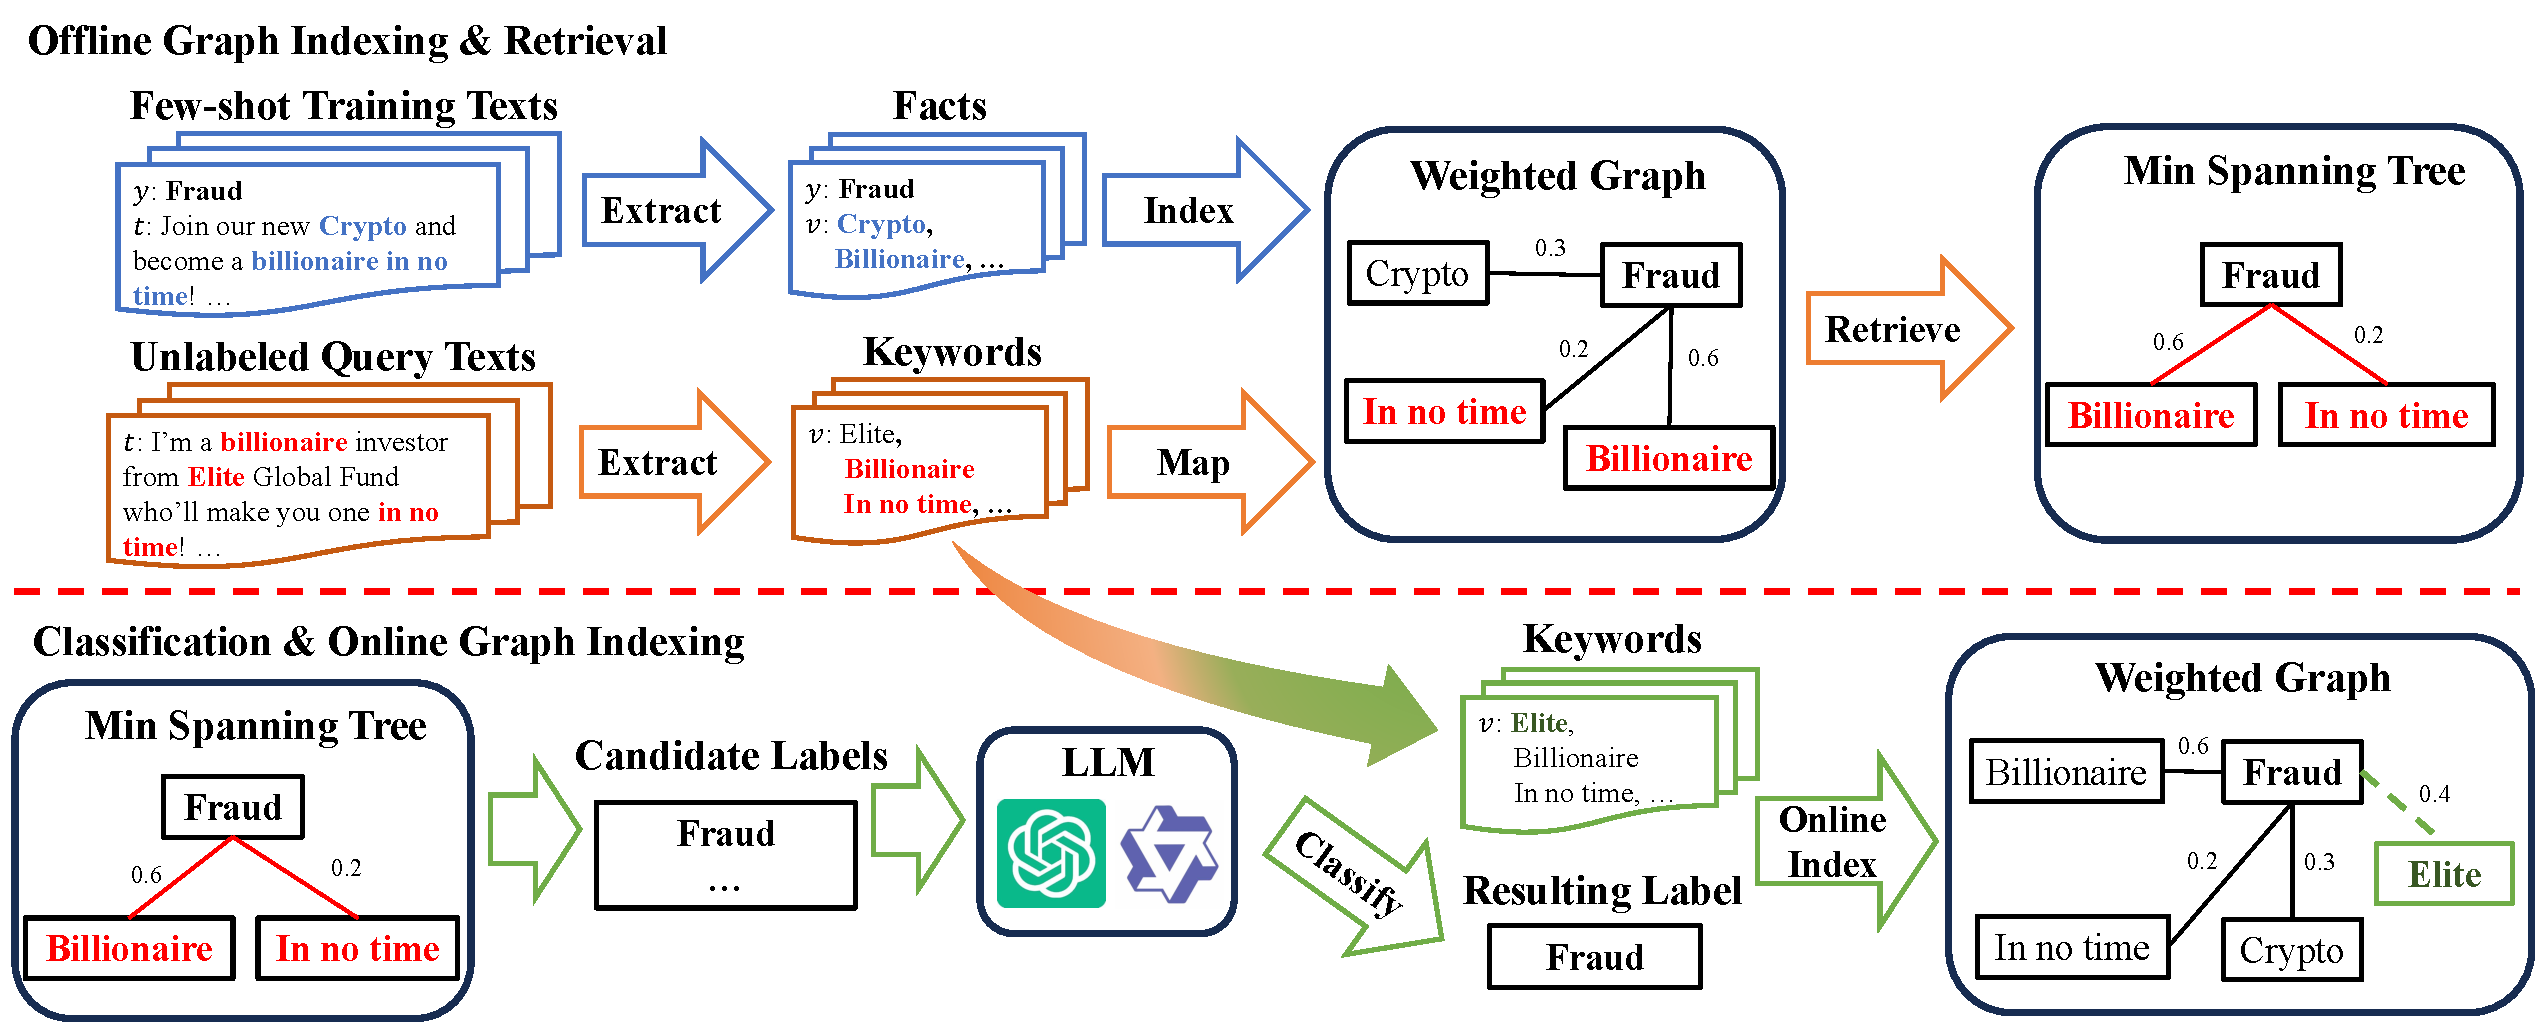
\includegraphics[width=\linewidth]{figures/gorag/GORAG_pipeline_example_new.pdf}
\caption{GORAG's offline indexing, query-dependent retrieval, classification, and online update. New query keywords are associated with the predicted class after classification. Reproduced from Figure 2 of GORAG~\cite{gorag-paper}.}
\label{fig:gorag:pipeline}
\end{figure}

\subsection{Keyword extraction and correlation scores}
\label{sec:gorag:keywords}

GORAG scores terms using normalized TF--IDF~\cite{gorag-tfidf}. Its extraction vocabulary includes words and phrases of fewer than three words. Let $\mathcal{T}_{\leq r}$ denote the corpus seen so far, and let $\operatorname{df}(v)$ be the number of its texts containing term $v$. The reported correlation score is
\begin{equation}
CS(v,t)=\frac{\operatorname{count}(v,t)}{|t|\log(|\mathcal{T}_{\leq r}|+1)}
\log\frac{|\mathcal{T}_{\leq r}|+1}{\operatorname{df}(v)+1}.
\label{eq:gorag:correlation}
\end{equation}
Here $\operatorname{count}(v,t)$ is the occurrence count of $v$ in $t$, and $|t|$ is text length. The expression combines frequency within the text with frequency across the observed corpus. Its corpus term changes when additional texts are observed. Terms with $CS(v,t)>\tau$ are retained, with $\tau=0.5$ in the original study. The method uses the score both to select keywords and to calculate association costs.
% Verification issue G5: source reports CS>tau with tau=0.5; normalization/threshold needs author/publication confirmation. Do not silently rescale.

A statistical extraction score gives each retained term a numerical contribution before graph retrieval. This contribution has a different role from the final language model's confidence in a label. The score determines which lexical units are indexed and how expensive their associations will be in retrieval. The evaluation of the full pipeline is therefore needed to establish the effect on classification.

Using short phrases can preserve a lexical combination that would be split by unigram indexing. At the same time, the extraction rule restricts what becomes a terminal later. Content absent from the extracted keyword set cannot directly act as a retrieval terminal for that query. The full query text remains available to the classifier, but its access to label evidence has already been shaped by the index representation. This relationship explains why extraction and classification should be described as separate stages.

\subsection{Keyword--label edge costs}
\label{sec:gorag:weights}

For keyword $v$ and label $y$, let $\mathcal{T}^{r,v,y}$ be the seen texts that contain $v$ and are associated with $y$. GORAG assigns the edge cost
\begin{equation}
w_{v,y}^r=\frac{\sum_{t_j\in\mathcal{T}^{r,v,y}}(1-CS(v,t_j))}{|\mathcal{T}^{r,v,y}|}.
\label{eq:gorag:weights}
\end{equation}
The complement converts a larger correlation score into a smaller contribution to connection cost. Averaging makes the edge depend on all contributing observations rather than on one occurrence. Offline observations use the supplied class of a support text; online observations use a predicted class when new query keywords are inserted.

An edge weight thus belongs to a particular keyword--label pair. It is not a global importance weight assigned to the keyword irrespective of class. The same keyword may occur in several label contexts, and the corresponding averages can differ. Retrieval uses the resulting cost structure together with connectivity. Replacing every cost by one preserves the graph's adjacency while removing this distinction, which is the purpose of the unit-weight ablation.

The averaging rule also identifies the granularity at which evidence is combined. Texts are not concatenated into one label description before the edge is scored. Each contributing text supplies a correlation value and the edge records their mean complement. A later text can contribute another occurrence to the associated pair. This design lets the index summarize recurrent lexical associations without putting every support text into each classification prompt.

\subsection{Merging label rounds}
\label{sec:gorag:merge}

At each round, the graph created from newly supplied information is merged with the graph accumulated from earlier rounds. The node and edge sets are unions. This operation retains the label universe already introduced while adding nodes and associations for the new task state. It differs from rebuilding a fresh graph containing only the most recently introduced labels, which would remove access to earlier alternatives.

GORAG also introduces edges between newly introduced and earlier label nodes. These bridges support connections between parts of the graph indexed in different rounds. Let $\mathcal{M}_y^r$ denote the keyword neighbors of label $y$. For a new label $y_n$ and an earlier label $y_o$, GORAG reports
\begin{equation}
w_{y_n,y_o}^r=\frac{1}{2}\left(
\frac{\sum_{v\in\mathcal{M}_{y_n}^r}w_{v,y_n}^r}{2|\mathcal{M}_{y_n}^r|}
+\frac{\sum_{v\in\mathcal{M}_{y_o}^r}w_{v,y_o}^r}{2|\mathcal{M}_{y_o}^r|}
\right).
\label{eq:gorag:labelbridge}
\end{equation}
The formula uses costs incident to both labels. These factors determine the relative cost of traversing a label bridge rather than a keyword association.
% Verification issue G6: preserve exact reported factors; source wording says weighted average.

Label bridges have a different evidential meaning from keyword--label edges. A keyword edge records a term's occurrence in texts associated with a class. A label bridge is added by the graph-merging procedure. It provides a connection through which retrieval can move between label regions. A retrieved path can therefore combine observed keyword associations with label bridges introduced during merging.

\section{Adaptive Candidate Label Retrieval}
\label{sec:gorag:retrieval}

For a query $t$, GORAG extracts keywords using the indexing procedure and partitions them according to whether they already occur in $\mathcal{V}^r$. Write these sets as $\mathcal{V}_{\mathrm{exist}}^t$ and $\mathcal{V}_{\mathrm{notexist}}^t$. The existing keywords become the terminals for current retrieval. The unseen keywords are held for online insertion after classification. The partition prevents the retrieval operation from treating an unindexed term as if it already had a known label neighborhood.

Retrieval seeks a low-cost connected structure that contains the mapped terminals. Label nodes encountered in this structure form the candidate set $\widehat{\mathcal{Y}}_t^r$. Connecting several terminals can select intermediate labels and keywords. The graph therefore determines the number of candidate labels through the returned structure, rather than requiring the same number of labels for all queries. A short query and a query containing several mutually distant indexed terms can produce different retrieval structures.

This terminal-connecting objective is related to the Steiner tree problem. In that problem, the required terminals are a subset of graph vertices, and the solution may use additional vertices to connect them. An ordinary minimum spanning tree instead spans all vertices of its input graph. These objects play distinct roles in GORAG's procedure. GORAG uses these intermediate structures to construct a heuristic connection among the query terminals.

\subsection{Tree and auxiliary-graph operations}
\label{sec:gorag:algorithm}

GORAG uses a greedy terminal-connecting procedure based on Mehlhorn's algorithm~\cite{gorag-mehlhorn1988faster}. The mapped keywords serve as terminals. An auxiliary graph $H$ represents connections between terminals, with edge weights given by path costs. A minimum spanning tree of $H$ selects a collection of terminal connections. Expanding these connections into their underlying paths produces the graph structure used for candidate selection. The language model then receives the labels encountered in this structure.

Once the expanded structure $S_t^r$ is obtained, the candidate set is
\begin{equation}
\widehat{\mathcal{Y}}_t^r=\mathcal{V}(S_t^r)\cap\mathcal{Y}^r.
\label{eq:gorag:candidates}
\end{equation}
Representative keywords and label descriptions are added to the classification prompt for the labels selected by this intersection.

\section{Classification and Online Indexing}
\label{sec:gorag:online}

GORAG constructs a classification input by concatenating the query text, extracted query keywords, retrieved candidate labels, and representative keywords associated with those labels. With $\mathcal{K}^t$ denoting query keywords and $\mathcal{K}_{\widehat{\mathcal{Y}}_t^r}$ the representative label information, the input is
\begin{equation}
c_t=\operatorname{Concat}\left(t,\mathcal{K}^t,\widehat{\mathcal{Y}}_t^r,\mathcal{K}_{\widehat{\mathcal{Y}}_t^r}\right).
\label{eq:gorag:context}
\end{equation}
A language model applies the classification instruction $p_{\mathrm{classify}}$ to this input and produces $y_t^*$. The graph narrows and describes the alternatives; the language model performs the final text classification.

Keeping the original query in this interface matters because keyword extraction removes ordering, local syntax, and surrounding discourse from the retrieval representation. The selected candidate set does not by itself determine how these features should affect the decision. The classifier can inspect the complete query alongside the retrieved label information. GORAG's keyword variant removes the full query from this input to test the contribution of that context under the same overall framework.

After the prediction, each keyword in $\mathcal{V}_{\mathrm{notexist}}^t$ is inserted into the graph and connected to $y_t^*$. The update can be written as
\begin{align}
\mathcal{V}^r&\leftarrow\mathcal{V}^r\cup\mathcal{V}_{\mathrm{notexist}}^t,\\
\mathcal{E}^r&\leftarrow\mathcal{E}^r\cup\{(v,y_t^*):v\in\mathcal{V}_{\mathrm{notexist}}^t\}.
\label{eq:gorag:update}
\end{align}
New associations receive weights through the reported weighting mechanism. Later queries can then map terms that were previously absent from the index. The update changes the retrieval source without fine-tuning the language model's parameters.

The prediction precedes insertion, so a new keyword's association can affect later queries but not the prediction that created it. Incorrect predicted labels can propagate through those associations. The offline ablation suppresses online expansion, measuring its contribution relative to an index that receives no such query-dependent additions.

\subsection{Computational organization}
\label{sec:gorag:computation}

The graph separates work performed at a label update from work performed for each query. Offline indexing processes the supplied texts, creates or updates keyword associations, generates label information when available, and merges the round's graph. The cross-round label bridges introduce interactions between the newly indexed and earlier label regions. In the source's abstract operation count, construction is expressed as
\begin{equation}
O\!\left(|\mathcal{Y}^r||\mathcal{Y}^{r-1}|+|\mathcal{V}_{\mathrm{new}}^r||\mathcal{D}^r|\right).
\label{eq:gorag:constructioncost}
\end{equation}
The two terms account for label merging and keyword--text processing. This count treats the associated text-processing and graph operations at the granularity used in that analysis. The number of tokens processed by a language-model call depends on the prompt and generated output, so the empirical token study supplies a separate measurement of model-facing work.

Per-query processing maps the extracted terms to the existing graph, obtains a connecting structure, builds the classification prompt, and inserts new terms after prediction. The index state can therefore grow during one round as well as between label rounds. Graph memory and prompt length measure different consequences of that growth. A larger stored index can provide more candidate associations while a query still receives only the labels selected by its own retrieval structure. The resource experiments report these two quantities separately.

\section{Experimental Design}
\label{sec:gorag:experiments}

The published study evaluates CAD, WOS, and IFS-Rel. CAD contains social media posts annotated for contextual abuse~\cite{gorag-vidgen2021introducing}. WOS contains academic texts associated with research-area labels~\cite{gorag-kowsari2017hdltex}. IFS-Rel supplies relation-classification examples derived from news text in an incremental few-shot benchmark~\cite{gorag-xia-etal-2021-incremental}. These datasets exercise different label vocabularies and text lengths within the dynamic classification setting.

The four-round split introduces 13 labels across CAD's rounds, 133 across WOS, and 64 across IFS-Rel. The test collections contain 817, 9,396, and 2,560 examples, respectively. IFS-Rel uses 40 test examples per label. Its balanced test allocation differs from the changing class frequencies in the other collections. Accuracy should therefore be interpreted with each dataset's actual split and distribution.

\begin{table}[tbp]
\centering
\caption{Dataset statistics for the four-round experiments, transposed from the original table. IFS-Rel has 40 test samples per label. Round label counts refer to newly introduced labels.}
\label{tab:gorag:dataset}
\small
\begin{tabular}{lrrr}
\hline
Statistic & CAD & WOS & IFS-Rel\\
\hline
Average text tokens & 154 & 200 & 105 \\
Round 1 test texts & 240 & 2,417 & 640 \\
Round 1 new labels & 4 & 32 & 16 \\
Round 2 test texts & 60 & 2,842 & 640 \\
Round 2 new labels & 3 & 53 & 16 \\
Round 3 test texts & 286 & 2,251 & 640 \\
Round 3 new labels & 3 & 30 & 16 \\
Round 4 test texts & 231 & 1,886 & 640 \\
Round 4 new labels & 3 & 18 & 16 \\
Total test texts & 817 & 9,396 & 2,560 \\
\hline
\end{tabular}
\end{table}


The label counts in Table~\ref{tab:gorag:dataset} describe labels introduced in each round. The classifier operates over their cumulative union. Thus the second WOS round adds 53 labels to the 32 labels already introduced, rather than replacing the earlier set by a new 53-label task. This distinction matters when relating the dataset statistics to the size of the classification instruction and to the graph state retained from earlier rounds.

The main few-shot study uses 1, 5, and 10 labeled examples per class. CAD and WOS RAG experiments use Qwen2.5-7B, while IFS-Rel uses GPT-4o. These are separate backbone conditions. The source reports an Intel Xeon Gold 5220R CPU at 2.20GHz and a single NVIDIA A100-SXM4-40GB GPU for the experiments. Runtime observations concern this implementation and hardware setting; API-backed inference also reflects the service used during the original study.

Classification accuracy requires an exact match between the model output and the ground-truth label name or number. An output that cannot be matched to the required class is not counted as correct. This protocol evaluates the final classification decision rather than a graded semantic similarity between arbitrary generated answers. A fluent explanation alone does not satisfy the metric.

\subsection{Compared methods and controls}
\label{sec:gorag:baselines}

The study compares six baselines. Entailment constructs text--label entailment pairs and fine-tunes a classifier~\cite{gorag-xia-etal-2021-incremental}. NaiveRAG retrieves text chunks from the indexed support information. Retrieved context is compressed by LongLLMLingua before classification~\cite{gorag-jiang-etal-2024-longllmlingua}. GraphRAG, LightRAG, and HippoRAG2 supply graph-based retrieval alternatives~\cite{gorag-edge2024local,gorag-guo2024lightrag,gorag-gutierrez2025memory}. Their classification results are measurements of the adaptations used in this study.

Entailment uses RoBERTa-large for five training epochs, a batch size of 16, a learning rate of $10^{-6}$, and Adam. LongLLMLingua is evaluated with compression rates of 0.75, 0.8, and 0.85, with 0.8 selected in the reported comparison. GraphRAG and LightRAG use local search. The source uses the nano-graphrag implementation for GraphRAG and NaiveRAG and the other baselines' official implementations. These choices identify the systems that produced the reported results.

The baseline collection tests several ways of allocating external context. NaiveRAG selects passages. LongLLMLingua changes which tokens remain in that context. The graph baselines select graph-associated information. GORAG explicitly selects labels through a connection structure and expands its lexical index online. These differences motivate the comparison, while the ablations isolate changes within GORAG's own pipeline more directly.

\section{Classification Results}
\label{sec:gorag:results}

The tables beginning with Tables~\ref{tab:gorag:main-wos} and~\ref{tab:gorag:main-ifs} preserve the WOS and IFS-Rel portions of the main accuracy table. Each dataset is split into one-, five-, and ten-shot tables, with rounds as columns. Each value is a fractional accuracy, and the labels available to the model expand with the round. The tables should be read by comparing methods under the same dataset, round, support size, and backbone.

% Layout split by shot; all 168 adopted WOS/IFS main cells retained.
\begin{table}[tbp]
\centering
\caption{WOS classification accuracy with one support example per label. Qwen2.5-7B is the RAG backbone. Values and emphasis reproduce the corresponding columns of GORAG's main table.}
\label{tab:gorag:main-wos}
\small
\begin{tabular}{lrrrr}
\hline
Method & Round 1 & Round 2 & Round 3 & Round 4\\
\hline
Entailment & {0.3695} & \underline{0.3994} & \underline{0.4510} & \underline{0.4030} \\
NaiveRAG & 0.3885 & 0.2267 & 0.1821 & 0.1653 \\
LongLLMLingua & 0.3806 & 0.2155 & 0.1770 & 0.1468 \\
GraphRAG & 0.3852 & 0.2213 & 0.1816 & 0.1641 \\
LightRAG & {0.3930} & 0.2202 & 0.1743 & 0.1625 \\
HippoRAG2 & \underline{0.4133} & 0.2552 & 0.2205 & 0.1906 \\
GORAG & \textbf{0.4866} & \textbf{0.4790} & \textbf{0.4736} & \textbf{0.4420} \\
\hline
\end{tabular}
\end{table}

\begin{table}[tbp]
\centering
\caption{WOS classification accuracy with 5 support examples per label. Qwen2.5-7B is the RAG backbone. Values and emphasis reproduce the corresponding columns of GORAG's main table.}
\label{tab:gorag:main-wos-5shot}
\small
\begin{tabular}{lrrrr}
\hline
Method & Round 1 & Round 2 & Round 3 & Round 4\\
\hline
Entailment & {0.3823} & \underline{0.4471} & \underline{0.4857} & \underline{0.4387} \\
NaiveRAG & {0.3904} & 0.2154 & 0.1475 & 0.1556 \\
LongLLMLingua & 0.3823 & 0.2202 & 0.1567 & 0.1382 \\
GraphRAG & 0.3897 & 0.2197 & 0.1770 & 0.1634 \\
LightRAG & 0.3806 & 0.2216 & 0.1767 & 0.1626 \\
HippoRAG2 & \underline{0.4245} & 0.2656 & 0.2210 & 0.1860 \\
GORAG & \textbf{0.4990} & \textbf{0.5109} & \textbf{0.4996} & \textbf{0.4717} \\
\hline
\end{tabular}
\end{table}

\begin{table}[tbp]
\centering
\caption{WOS classification accuracy with 10 support examples per label. Qwen2.5-7B is the RAG backbone. Values and emphasis reproduce the corresponding columns of GORAG's main table.}
\label{tab:gorag:main-wos-10shot}
\small
\begin{tabular}{lrrrr}
\hline
Method & Round 1 & Round 2 & Round 3 & Round 4\\
\hline
Entailment & {0.4187} & \underline{0.4222} & \underline{0.4787} & \underline{0.4442} \\
NaiveRAG & 0.3897 & 0.2187 & 0.1799 & 0.1649 \\
LongLLMLingua & 0.3901 & 0.2198 & 0.1608 & 0.1493 \\
GraphRAG & 0.3906 & 0.2219 & 0.1786 & 0.1625 \\
LightRAG & 0.3815 & 0.2145 & 0.1799 & 0.1632 \\
HippoRAG2 & \underline{0.4208} & 0.2666 & 0.2242 & 0.1915 \\
GORAG & \textbf{0.5134} & \textbf{0.5284} & \textbf{0.5234} & \textbf{0.4929} \\
\hline
\end{tabular}
\end{table}

\begin{table}[tbp]
\centering
\caption{IFS-Rel classification accuracy with one support example per label. GPT-4o is the RAG backbone. Values and emphasis reproduce the corresponding columns of GORAG's main table.}
\label{tab:gorag:main-ifs}
\small
\begin{tabular}{lrrrr}
\hline
Method & Round 1 & Round 2 & Round 3 & Round 4\\
\hline
Entailment & 0.3391 & {0.4008} & {0.3061} & {0.2971} \\
NaiveRAG & {0.7343} & 0.5394 & \underline{0.4719} & 0.5233 \\
LongLLMLingua & \underline{0.8750} & \underline{0.5734} & 0.4703 & \underline{0.5819} \\
GraphRAG & 0.6406 & 0.4406 & 0.3828 & 0.4297 \\
LightRAG & 0.7578 & 0.4906 & 0.3802 & 0.4531 \\
HippoRAG2 & 0.7313 & 0.4875 & 0.4297 & 0.4984 \\
GORAG & \textbf{0.9688} & \textbf{0.5938} & \textbf{0.4844} & \textbf{0.6165} \\
\hline
\end{tabular}
\end{table}

\begin{table}[tbp]
\centering
\caption{IFS-Rel classification accuracy with 5 support examples per label. GPT-4o is the RAG backbone. Values and emphasis reproduce the corresponding columns of GORAG's main table.}
\label{tab:gorag:main-ifs-5shot}
\small
\begin{tabular}{lrrrr}
\hline
Method & Round 1 & Round 2 & Round 3 & Round 4\\
\hline
Entailment & {0.6046} & {0.5516} & {0.4703} & {0.4395} \\
NaiveRAG & 0.7344 & 0.5406 & 0.4719 & {0.4938} \\
LongLLMLingua & \underline{0.8906} & \underline{0.5922} & \underline{0.4741} & 0.4903 \\
GraphRAG & 0.7813 & 0.4688 & 0.3734 & 0.4422 \\
LightRAG & 0.8281 & 0.5155 & 0.4010 & 0.4804 \\
HippoRAG2 & 0.7375 & 0.5016 & 0.4328 & \underline{0.5008} \\
GORAG & \textbf{0.9688} & \textbf{0.6172} & \textbf{0.4948} & \textbf{0.4988} \\
\hline
\end{tabular}
\end{table}

\begin{table}[tbp]
\centering
\caption{IFS-Rel classification accuracy with 10 support examples per label. GPT-4o is the RAG backbone. Values and emphasis reproduce the corresponding columns of GORAG's main table.}
\label{tab:gorag:main-ifs-10shot}
\small
\begin{tabular}{lrrrr}
\hline
Method & Round 1 & Round 2 & Round 3 & Round 4\\
\hline
Entailment & {0.5859} & \underline{0.5828} & {0.5193} & {0.4895} \\
NaiveRAG & 0.7406 & 0.5469 & 0.4688 & 0.5000 \\
LongLLMLingua & \underline{0.9219} & 0.5806 & \underline{0.5225} & \underline{0.5038} \\
GraphRAG & 0.8125 & 0.4719 & 0.3141 & 0.3922 \\
LightRAG & 0.8594 & 0.5156 & 0.4427 & 0.4610 \\
HippoRAG2 & 0.7406 & 0.4938 & 0.4438 & 0.4953 \\
GORAG & \textbf{0.9688} & \textbf{0.6250} & \textbf{0.5344} & \textbf{0.5469} \\
\hline
\end{tabular}
\end{table}


On WOS with one support example per label, GORAG reports accuracies of 0.4866, 0.4790, 0.4736, and 0.4420 across the four rounds. Entailment reports 0.3695, 0.3994, 0.4510, and 0.4030 in the same columns. The corresponding GraphRAG values are 0.3852, 0.2213, 0.1816, and 0.1641. These comparisons locate the result in a setting where the number of candidate labels increases substantially over the evaluation.

Additional support examples improve GORAG's WOS accuracy in the main table. At the fourth round, its one-, five-, and ten-shot values are 0.4420, 0.4717, and 0.4929. At the first round they are 0.4866, 0.4990, and 0.5134. The changing label universe and changing support size are separate experimental axes. 

IFS-Rel uses GPT-4o. In its first round, GORAG reports 0.9688 for all three support sizes, while the fourth-round scores are 0.6165, 0.4988, and 0.5469. The five-shot fourth-round value is below the one-shot value, so increasing support size does not produce a monotonic improvement in every setting. LongLLMLingua reports 0.5819, 0.4903, and 0.5038 in these fourth-round columns. HippoRAG2 reports 0.4984, 0.5008, and 0.4953; its five-shot result exceeds GORAG's five-shot result in that column.

CAD uses Qwen2.5-7B. Its GORAG first-round accuracy is 0.6125 in all three support settings. The fourth-round one- and five-shot accuracies are 0.3133 and 0.3146. Accuracy decreases in later rounds as the cumulative label set grows. 
% G2: full CAD table withheld from integrated chapter because source CAD/R4/10-shot is literal 03139. Exact working transcription in planning/gorag-working-cad-table.tex.

WOS improves with additional support in the displayed rounds, whereas IFS-Rel is non-monotonic across support sizes and CAD loses accuracy as labels accumulate.

\section{Ablations and Resource Use}
\label{sec:gorag:ablations}

The WOS ablation study uses a one-shot Qwen2.5-7B setting. The offline variant disables online indexing. The unit variant assigns cost one to every graph edge. The offline-and-unit variant removes both features. The keyword variant uses the extracted keywords in place of the complete query text for classification. These variants change specific inputs or index operations while retaining GORAG's overall classification task.

% Exact active-source transcription, numerical values retained.
\begin{table}[t]
	\centering
	\caption{Ablation experiments on WOS for GORAG's variants.}
	
	\label{tab:gorag:ablation}
	\small
		\begin{tabular}{l|l|c|c|c|c} 
			\hline\hline
			\multirow{2}{*}{\textbf{Dataset}} & \multirow{2}{*}{\textbf{Model}} & \multicolumn{4}{c}{\textbf{Round}}                                        \\ 
			\cline{3-6}
			& & R1              & R2         & R3           & R4  \\ 
			\hline
			\multirow{5}{*}{\textbf{WOS}} 
			& GORAG \textit{offline\&unit}          &     0.2979            &     0.2287            &       0.2645          &      0.2249                        \\
			& GORAG \textit{offline}          &     0.3063            &     0.2302            &       0.2455          &      0.2156                        \\
			&  GORAG \textit{unit}             & 0.4706          & 0.4394          & 0.4407          & 0.3899                      \\
			& GORAG \textit{keyword}         & \underline{0.4746}          & \underline{0.4606}          & \underline{0.4455}          & \underline{0.4030}             \\ 
			& \textbf{GORAG}                           & \textbf{0.4862}          &  \textbf{0.4649}              &     \textbf{0.4814}            &       \textbf{0.4210}                    \\
			\hline\hline
			
			
			
			
			
			
		\end{tabular}
	
\end{table}


In the ablation table, the full method reports 0.4862, 0.4649, 0.4814, and 0.4210 across rounds. The offline variant reports 0.3063, 0.2302, 0.2455, and 0.2156. The unit variant reports 0.4706, 0.4394, 0.4407, and 0.3899. Under this ablation protocol, removing online insertion has a larger observed effect than replacing the weighted graph with unit costs. This comparison concerns the variants reported together in that table.

The offline-and-unit variant reports 0.2979, 0.2287, 0.2645, and 0.2249. Its third- and fourth-round values exceed those of the offline variant. The effects of removing these components are therefore not strictly additive across rounds. The keyword variant reports 0.4746, 0.4606, 0.4455, and 0.4030, below the full method in each displayed column. The full query provides information useful to the classifier in these experiments even though keywords determine the retrieval terminals.

The publication gives different full-method values in the main and ablation WOS tables without explaining their provenance. Component comparisons here use the full-method row from the ablation table.

\subsection{Prompt tokens and graph growth}
\label{sec:gorag:resources}

The IFS-Rel one-shot token study reports average tokens per query and the corresponding US-dollar costs under the original study's pricing conditions. GORAG uses 557.5 tokens per query and reports a cost of \$0.004. The direct GPT-4o comparison uses 634.6 tokens and reports \$0.005. LongLLMLingua uses 2,771.3 tokens, NaiveRAG 4,537.4, LightRAG 7,866.3, and GraphRAG 9,296.3. Their reported costs are \$0.021, \$0.034, \$0.059, and \$0.070, respectively.

% Exact active-source transcription, numerical values retained.
\begin{table}[t]
	\centering
	\caption{Token cost on IFS-Rel dataset with 1-shot setting.}
	\label{tab:gorag:token}
	
	\small
		\begin{tabular}{l|c|c} 
			\hline\hline
			\textbf{Model} & \textbf{AVG Token per Query} & \textbf{AVG Cost per Query (USD)}  \\ 
			\hline
			GPT-4o         & 634.6                        & \$0.005                               \\
			LongLLMLingua  & 2771.3                       & \$0.021                               \\
			NaiveRAG       & 4537.4                       & \$0.034                               \\
			LightRAG       & 7866.3                       & \$0.059                               \\
			GraphRAG       & 9296.3                       & \$0.070                               \\
			\textbf{GORAG} & \textbf{557.5}               & \textbf{\$0.004}                      \\
			\hline\hline
		\end{tabular}
	
\end{table}


The token comparison measures how much context reaches the model in the evaluated implementation. GORAG's candidate-label representation uses fewer tokens than the listed retrieval baselines in this experiment. The historic dollar values provide the cost calculation reported with those measurements; they are not current API price quotations. Token totals and monetary costs should remain attached to this IFS-Rel one-shot protocol when discussing efficiency.

Graph growth is measured separately during the first IFS-Rel round with GPT-4o. The reported index contains 1,644 nodes and 1,771 edges at the 25-percent checkpoint, and 5,299 nodes and 5,503 edges at the final checkpoint. The corresponding reported memory values are 13.3 KB and 46.4 KB. These measurements concern the graph representation in that experiment. They do not include the complete memory required to host or serve the language model.
% G3: original intermediate node-count increment annotation is inconsistent; complete graph-growth table withheld pending clarification.

The original runtime study compares total time on WOS and CAD under the one-shot setting, using Qwen2.5-7B. Its figures belong to those dataset and hardware conditions. Online insertion adds work after each prediction, while statistical keyword indexing and smaller model inputs can change other parts of the pipeline. Runtime must therefore be measured end to end rather than inferred from token counts alone. This chapter retains the separation between prompt-token evidence, graph-memory evidence, and the source's total-time experiment.

\begin{figure}[tbp]
\centering
\begin{minipage}{0.48\linewidth}\centering
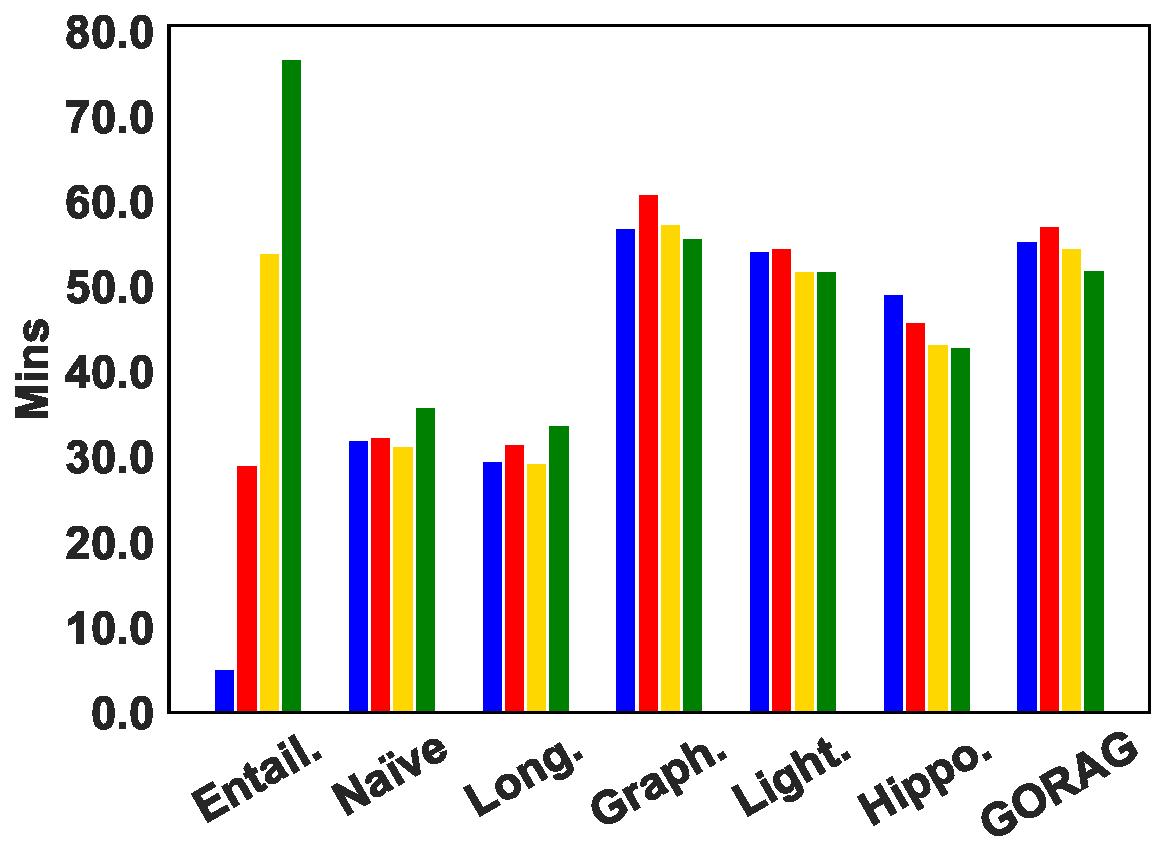
\includegraphics[width=\linewidth]{figures/gorag/runtime_wos.pdf}\par (a) WOS.
\end{minipage}\hfill
\begin{minipage}{0.48\linewidth}\centering
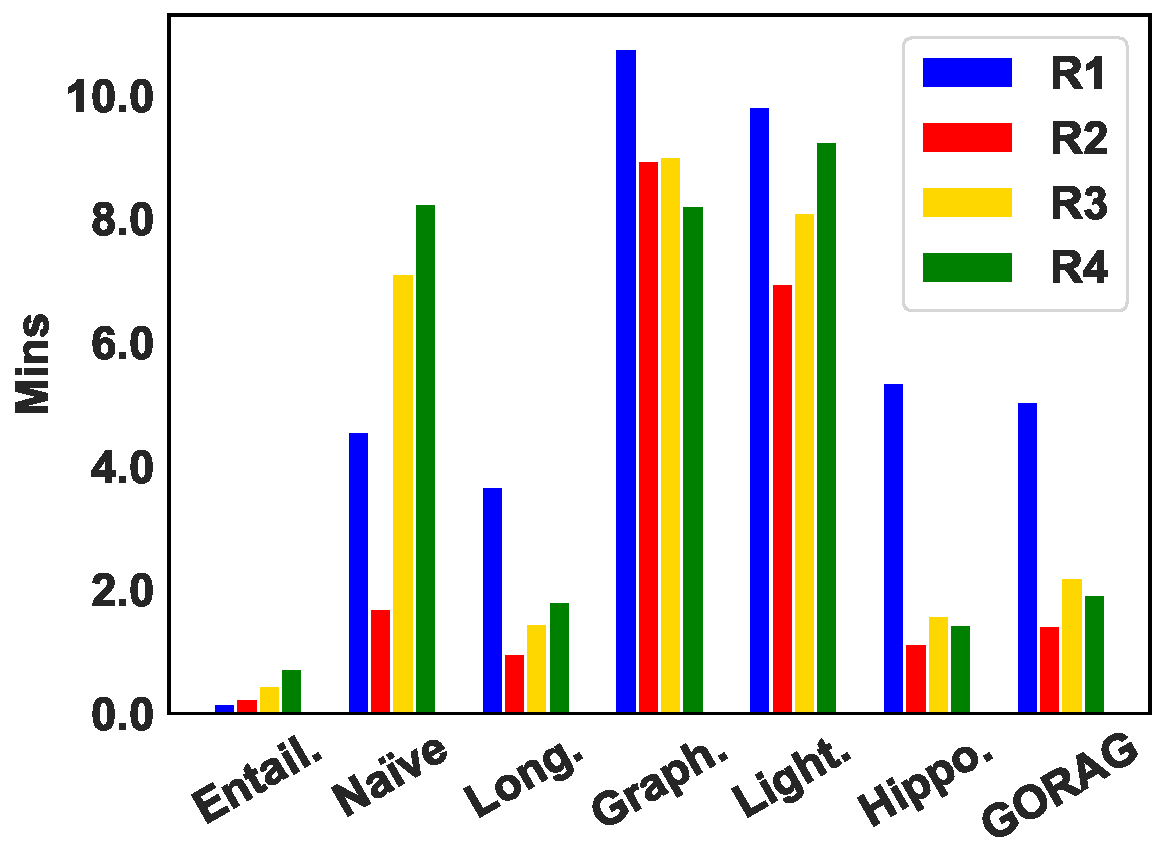
\includegraphics[width=\linewidth]{figures/gorag/runtime_cad.pdf}\par (b) CAD.
\end{minipage}
\caption{Total time in minutes for the one-shot four-round experiments with Qwen2.5-7B. The original R1--R4 legend in panel (b) applies to both panels. Reproduced from Figure 3 of GORAG~\cite{gorag-paper}.}
\label{fig:gorag:runtime}
\end{figure}

\section{Zero-shot and Round Generalization}
\label{sec:gorag:generalization}

The zero-shot IFS-Rel experiment supplies label names and language-model-generated descriptions without annotated support texts. GORAG extracts keywords from these descriptions to initialize its graph. The experiment consequently tests whether description-derived associations can support candidate selection and subsequent classification.

% Exact active-source transcription, numerical values retained.
\begin{table}[t]
	\centering
	\caption{0-shot experiments for GORAG and RAG baselines on IFS-Rel dataset under 0-shot setting.}
	\label{tab:gorag:zero}
	
	\small
		\begin{tabular}{l|c|c|c|c} 
			\hline\hline
			\textbf{Model}          & \textbf{R1}              & \textbf{R2}              & \textbf{R3}              & \textbf{R4}               \\ 
			\hline
			GPT-4o \cite{gorag-hurst2024gpt}                  & 0.9219                   & 0.5109                   & 0.4063                   & \underline{0.5936}                    \\ 
			LongLLMLingua \cite{gorag-jiang-etal-2024-longllmlingua}          & \underline{0.9281}                   & \underline{0.5297}                   & \underline{0.4234}                   & 0.5806                    \\
			LightRAG \cite{gorag-guo2024lightrag}                & 0.6718                   & 0.3047                   & 0.2135                   & 0.0977                    \\ 
			GraphRAG \cite{gorag-edge2024local}                & 0.5625                   & 0.1875                   & 0.1458                   & 0.0938                    \\
			\textbf{\textbf{GORAG}} & \textbf{\textbf{0.9328}} & \textbf{\textbf{0.5406}} & \textbf{\textbf{0.4375}} & \textbf{\textbf{0.6063}}  \\
			\hline\hline
		\end{tabular}
	
\end{table}


GORAG reports zero-shot accuracies of 0.9328, 0.5406, 0.4375, and 0.6063. The direct GPT-4o comparison reports 0.9219, 0.5109, 0.4063, and 0.5936. LongLLMLingua reports 0.9281, 0.5297, 0.4234, and 0.5806. The graph-based comparisons in the same table are lower under this initialization protocol. These values support the use of label descriptions as an initial retrieval source for this experiment.

The round-generalization study uses WOS split into four, six, and eight rounds under one- and five-shot settings. The displayed curve combines rounds one to four from the four-round split, rounds five and six from the six-round split, and rounds seven and eight from the eight-round split. These points represent results from different partitions of the label set. They do not form the trajectory of one index updated through eight consecutive rounds.

\begin{figure}[tbp]
\centering
\begin{minipage}{0.48\linewidth}\centering
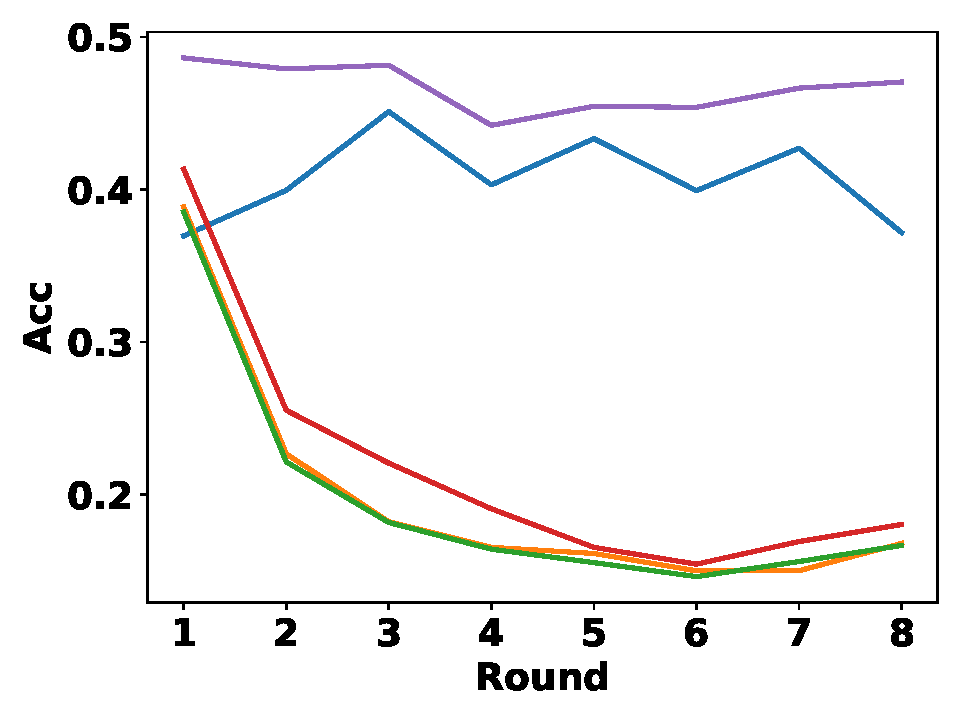
\includegraphics[width=\linewidth]{figures/gorag/wos_4_round_1.pdf}\par (a) One-shot.
\end{minipage}\hfill
\begin{minipage}{0.48\linewidth}\centering
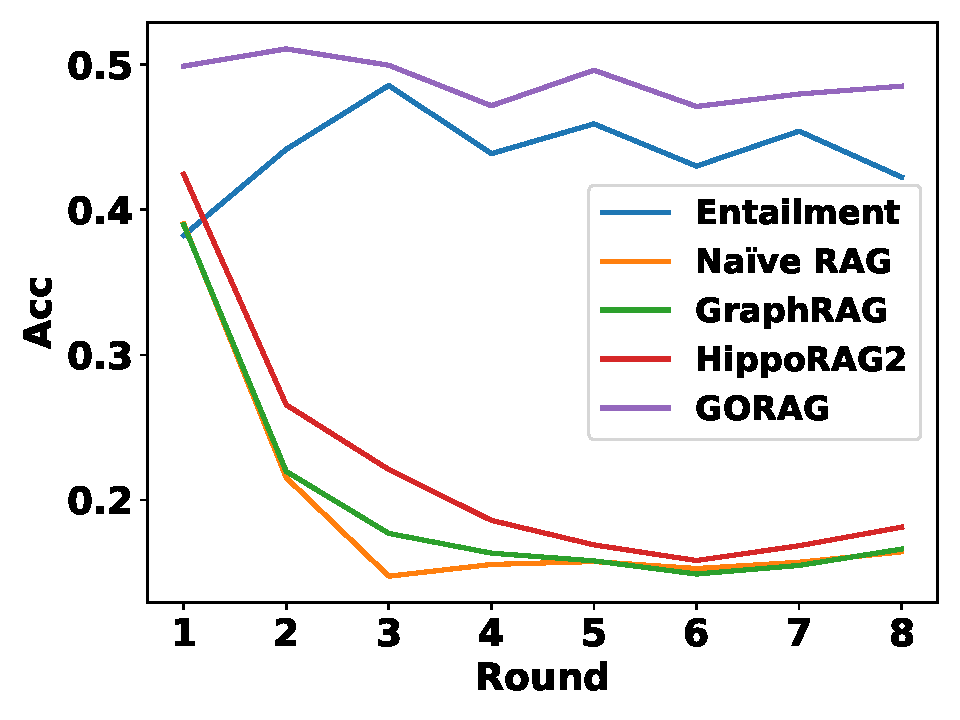
\includegraphics[width=\linewidth]{figures/gorag/wos_4_round_5.pdf}\par (b) Five-shot.
\end{minipage}
\caption{WOS classification across the reported round splits. Points 1--4 use the four-round split, 5--6 the six-round split, and 7--8 the eight-round split. The legend in panel (b) applies to both panels. Reproduced from Figure 4 of GORAG~\cite{gorag-paper}.}
\label{fig:gorag:rounds}
\end{figure}

\subsection{A retrieved classification case}
\label{sec:gorag:case}

Figure~\ref{fig:gorag:case} reproduces a contextual-abuse example from the original study. The query contains the terms highlighted in red. These terms map to keyword nodes, and the selected connecting structure passes through an insult label. The classifier outputs the abuse category shown in the figure. This example exposes the relationship between the extracted query evidence, the intermediate label node, and the final classification.

The useful property of the example is that candidate selection has a visible provenance. The label is connected to more than one term in the indexed representation. The displayed nonterminal neighbor also shows that a keyword neighborhood can contain more information than the connection chosen for the current text. Selecting a structure distinguishes the evidence used to connect the query terms from other associations present around the same label.

\begin{figure}[tbp]
\centering
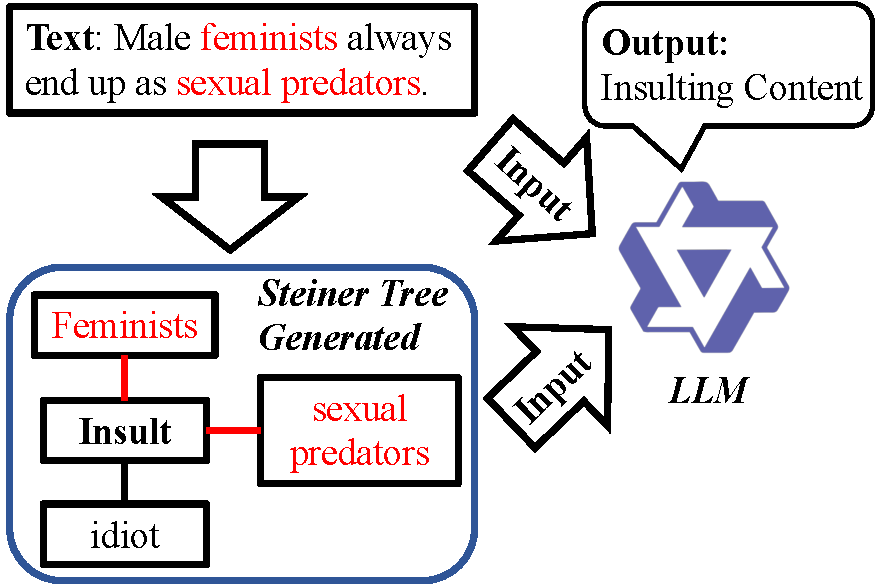
\includegraphics[width=0.75\linewidth]{figures/gorag/new_case.pdf}
\caption{A contextual-abuse example and its selected graph connections. Reproduced from Figure 5 of GORAG~\cite{gorag-paper}.}
\label{fig:gorag:case}
\end{figure}

\section{Discussion and Chapter Summary}
\label{sec:gorag:discussion}

GORAG places structure between the observation of text and the construction of a language model's classification instruction. Keywords connect the current text to an accumulated graph. Edge costs and terminal connections select a subset of label alternatives. The model then classifies the original text with these alternatives and their representative information. Structure serves as a task-specific evidence-selection mechanism.

The offline ablation shows the contribution of expanding the index beyond the support sample. Because these additions carry predicted labels, the method couples current classification with the evidence available to later queries.

The graph's paths provide a trace of the index connections used for retrieval. They can reveal which keywords and labels were linked by the selected structure. This trace explains the provenance of candidate selection in the constructed graph. The final classifier still receives text and makes a language-model prediction; the retrieved path is an external evidence object rather than an observation of the model's internal computation.

Several conditions bound the interpretation of the chapter's evidence. Keyword extraction determines which parts of a query can become terminals. Sparse support data and limited label descriptions determine initial coverage. Predicted-label insertion can add incorrect associations. The accuracy tables use exact label matching and different backbones for different datasets. Each condition identifies a concrete component or evaluation choice that affects the reported classification result.

Within these conditions, the study shows how a task graph can reduce the label-selection burden placed on a language model and maintain lexical evidence as the task evolves. The contribution differs from KGLink's use of an existing knowledge graph to enrich table representations. Here the structure is built and updated from task data, and its immediate output is a query-specific label set. The next chapter turns from choosing among labels to selecting connected textual facts for an open-ended answer. That change requires a retrieval objective that accounts for the relevance and connection cost of evidence beyond a fixed classification vocabulary.
